\documentclass{article}

\usepackage[utf8]{inputenc}

\usepackage{color}
\usepackage{amsmath}
\usepackage{amsfonts}
\usepackage{amssymb}
\usepackage{amsthm}
\usepackage{mathabx}
\usepackage{geometry}
\usepackage{graphicx}
\usepackage{pgf}
\usepackage{tikz}

\geometry{
	b5paper,
	margin=1.5cm,
	top=1.75cm,
	bottom=1.75cm
}

\newcommand{\llinnm}[2]{\operatorname{L}_{\operatorname{lin}}({#1}, {#2})}
\newcommand{\llinn}[1]{\llinnm{#1}{#1}}
\newcommand{\hlinr}[1]{\operatorname{H}_{\operatorname{lin}}^{#1}}
\newcommand{\hlin}{\operatorname{H}_{\operatorname{lin}}}
\newcommand{\leap}[3]{\operatorname{\mathbf{leap}}({#1}, {#2}, {#3})}
\newcommand{\hfact}[2]{\operatorname{H}_{\operatorname{factor}}({#1}, {#2})}
\newcommand{\rot}[2]{\operatorname{H}_{\operatorname{rot}}^{{#1}, {#2}}}

\newcommand{\bin}[3]{\operatorname{\mathbf{bin}}({#1}, {#2}, {#3})}
\newcommand{\lbin}[2]{\operatorname{\mathbf{lbin}}({#1}, {#2})}
\newcommand{\vbin}[2]{\operatorname{\mathbf{bin}}({#1}, {#2})}
\newcommand{\vlbin}[1]{\operatorname{\mathbf{lbin}}({#1})}

\newcommand{\vecspace}[2]{\mathbb{Z}_{#1}^{#2}}
\newcommand{\binvecspace}[1]{\vecspace{2}{#1}}
\newcommand{\linearmaps}[2]{\mathcal{L}_{#1}^{#2}}
\newcommand{\surjectivelinearmaps}[2]{\mathcal{LS}_{#1}^{#2}}

\newcommand{\probs}[2]{\operatorname{\mathbf{Pr}}_{{#1}}\left[{#2}\right]}
\newcommand{\prob}[1]{\probs{}{#1}}
\newcommand{\expects}[2]{\operatorname{\mathbf{E}}_{{#1}}\left[{#2}\right]}
\newcommand{\expect}[1]{\expects{}{#1}}
\newcommand{\inu}{\in_U}

\newtheorem{lemma}{Lemma}
\newtheorem{definition}{Definition}
\newtheorem{theorem}{Theorem}
\newtheorem{claim}{Claim}
\newtheorem{corollary}{Corollary}

\title{An upper bound on the size of the largest bin using linear transformations over vector spaces}

\author{Martin Babka}

\begin{document}

\maketitle

\begin{abstract}
We improve the proof of Alon et al. to show that the size of the largest bin when hashing $n$ balls into $n$ bins is $O(\log n)$. This improves the currently known upper bound which is $O(\log n \log \log n)$ for hashing $n \log n$ balls into $n$ bins.
\end{abstract}

\section{Setting and notation}
By $\linearmaps{u}{b}$ we denote all linear transformations from $\binvecspace{u}$ to $\binvecspace{b}$.
By $\surjectivelinearmaps{u}{b}$ we denote all surjective linear transformations from $\binvecspace{u}$ onto $\binvecspace{b}$.
Let $S \subseteq \binvecspace{u}$ and $T \in \linearmaps{u}{b}$. By $\lbin{T}{S}$ we denote $\operatorname{argmax}_{y \in \binvecspace{b}} |T^{-1}(y) \cap S|$.

\section{The size of the largest bin with the linear transformations}

We are dealing with the situation of placing $n$ balls, i.e. $n$ vectors, into $n$ bins.
We prove that in such case the size of the largest bin is $O(\log n)$. 
This improves the current best result which holds for placing $n \log n$ balls into $n$ bins and bounds the size of the largest bins by $O(\log n \log \log n)$.
In the setting for $n$ balls this improves the best known result by  $\log \log n$ factor.
\begin{theorem}
\label{theorem-n-to-n}
Let $S \subset \binvecspace{u}$ and let $n = |S|$. It holds that $\expects{T \in_U \linearmaps{u}{\log n}}{\lbin{T}{S}} = O(\log n)$.
\end{theorem}
We proceeded in the same way as in \cite{alonetal} we just switch to a different parametrization.
Let us cite several results from \cite{alonetal} which are reused in our proof and thus are not proven here.
\begin{theorem}
\label{theorem-prob-bound}
Let $t, u \in \mathbb{N}$, $t < u$.
Let $S \subseteq \binvecspace{u}$ such that $\alpha = 1 - \frac{|S|}{2^u}$, $\alpha < 1$.
Then 
\[
\probs{T \in_U \surjectivelinearmaps{u}{t}}{T(S) \neq \binvecspace{t}} \leq \alpha^{u - t - \log t + \log \log \frac{1}{\alpha}}.
\]
\end{theorem}
\begin{proof}
Theorem~{7b} from \cite{alonetal}.
\end{proof}

\begin{theorem}
\label{theorem-epsilon}
Let $t \in \mathbb{N}$.
Then for each $\epsilon > 0$ exists $c_\epsilon > 0$ such that for each $S \subset \binvecspace{u}$, $|S| \geq c_\epsilon t 2^t$ it holds  $\probs{T \in_U \linearmaps{u}{t}}{T(S) = \binvecspace{t}} \geq 1 - \epsilon$.
\end{theorem}
\begin{proof}
Theorem~{7a} from \cite{alonetal}.
\end{proof}

We now define the same two events as in \cite{alonetal}.
The first one, $E_1$, occurs if there is a chain of length at least $l$.
The second one, $E_2$ is used to bound the probability of occurrence of  $E_1$.
\begin{definition}
Let $l \in \mathbb{N}$, $T \in \linearmaps{u}{b}$. We define $E_1(S, T, l)$ as $\exists \vec{y} \in \binvecspace{b} \colon |T^{-1}(y) \cap S| \geq l$.
\end{definition}

We redefine event $E_2$ from \cite{alonetal}. 
This event occurs along with $E_1$ with a constant probability as is analyzed later in the text. 
Using this fact we may bound the probability of $E_1$ by bounding the probability of occurrence of $E_2$. 
To define $E_2$ we factor the linear map $T \in \linearmaps{u}{b}$ through a factor vector space $\binvecspace{f}$ into two linear maps $T_0 \in \linearmaps{u}{f}$ and $T_1 \in \surjectivelinearmaps{f}{b}$ satisfying that $T = T_0 \circ T_1$.
\begin{definition}
Let $u, f, b \in \mathbb{N}$, $f \geq b$, $S \subseteq \binvecspace{u}$, $T_0 \in \linearmaps{u}{f}$ and $T_1 \in \surjectivelinearmaps{f}{b}$.
The event $E_2(S, T_0, T_1)$ occurs when $\exists \vec{y} \in \binvecspace{b} \colon T_1^{-1}(y) \subseteq T_0(S)$.
\end{definition}

From now on we assume that $u, f, b \in \mathbb{N}$, $f \geq b$, $S \subseteq \binvecspace{u}$, $T_0 \in_U \linearmaps{u}{f}$ and $T_1 \in_U \surjectivelinearmaps{f}{b}$. 
For the main linear map $T \in_U \linearmaps{u}{b}$ it holds that $T = T_0 \circ T_1$.

\begin{lemma}
\label{lemma-e1-e2}
Assume that $T$ and $T_1$ are fixed and $T_0$ is fixed except for the mapping $T_k$ between the kernel of $T_0$ and $T_1$.
For each $\epsilon > 0$ there is $c_\epsilon > 0$ such that if $l \geq c_\epsilon (f - b)2^{f-b}$, then
\[
\probs{T_k \in_u \linearmaps{\operatorname{dim}(\operatorname{Ker}(T))}{f-b}}{E_2(S, T_0, T_1) | E_1(S, T, l)} \geq 1 - \epsilon.
\]
\end{lemma}
\begin{proof}
Assume that $E_1(S, T, l)$ occurs. 
Then there is $\vec{y} \in \binvecspace{b}$ such that $|T^{-1}(y) \cap S| \geq l$.
Put $U_A = T^{-1}(\vec{y})$, $S_A = U_A \cap S$ and $F_A = T_1^{-1}(\vec{y})$.
Notice that $|F_A| = 2^{f-b}$ and $|S_A| = l$.
Moreover $U_A$ and $F_A$ are affine subspaces of $\binvecspace{u}$ and $\binvecspace{f}$.
Using Theorem~\ref{theorem-epsilon} for $U_A$, $S_A$, $F_A$ and $T_k$ yields the wanted statement since if $T_k^A(S_A) = F_A$\footnote{$T_k^A$ is the affine linear map between $U_A$ and $F_A$ completely defined by $T_k$.}, then $E_2$  occurs.
\end{proof}

\begin{figure}[h]
	\caption{The general case of the factorization of $T$.}

\begin{center}
	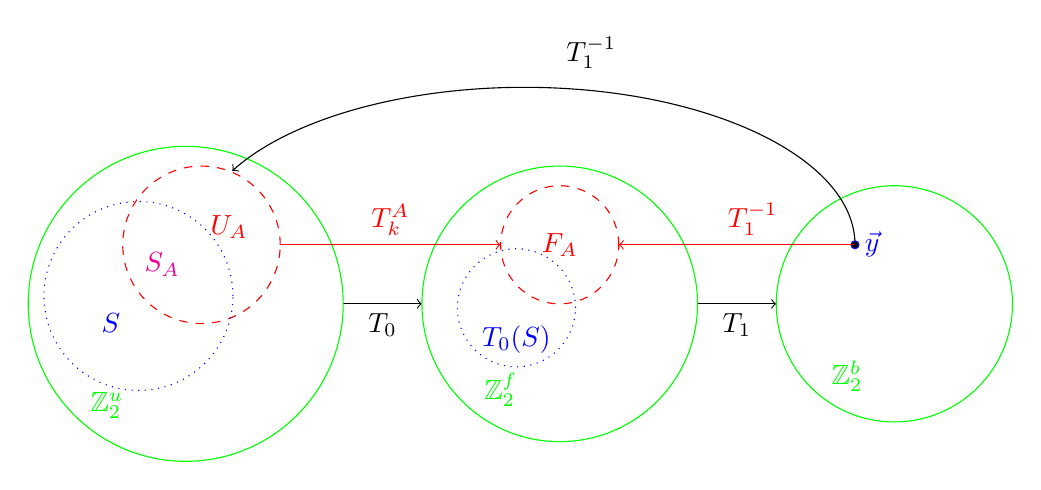
\begin{tikzpicture}
		\draw[->] (4,2) -- (5,2) node[left=0.5cm,below] {$T_0$};
		\draw[green] (2,2) circle (2cm) node[left=1cm,below=1cm] {$\binvecspace{u}$};
		\draw[green] (6.75,2) circle (1.75cm) node[left=0.75cm,below=0.75cm] {$\binvecspace{f}$};
		\draw[->] (8.5,2) -- (9.5,2) node[left=0.5cm,below] {$T_1$};
		\draw[green] (11,2) circle (1.5cm) node[left=0.6cm,below=0.6cm] {$\binvecspace{b}$};
		
		\draw[blue] (10.5,2.75) circle (0.05cm) [fill=black] node[anchor=west] {$\vec{y}$};
		\draw[->,red] (10.5,2.75) -- (7.5,2.75) node[left=-1.7cm,above] {$T_1^{-1}$};
		\draw[dashed,red] (6.75,2.75) circle (0.75cm)  node[] {$F_A$};
		\draw[dotted,blue] (6.2,1.95) circle (0.75cm)  node[left=0cm,below=0.1cm] {$T_0(S)$};

		\draw[dashed,red] (2.2,2.75) circle (1cm)  node[left=-0.35cm,below=-0.5cm] {$U_A$};
		\draw[dotted,blue] (1.4,2.1) circle (1.2cm)  node[left=0.35cm,below=0.1cm] {$S$};
		
		\draw[magenta] (1.7,2.5) node[] {$S_A$};
		

		\draw[->] (10.5,2.75) arc (0:152:4.2cm and 2cm) node[below=-1.5cm,left=-5cm] {$T_1^{-1}$};
		
		
		\draw[->,red] (3.2,2.75) -- (6,2.75) node[left=1.4cm,above] {$T_k^A$};
	\end{tikzpicture}
\end{center}
\end{figure}

\begin{figure}
	\caption{Event $E_2(S, T_0, T_1)$ occurs, i.e. $F_A \subseteq T_0(S)$. Notice that $T_1(T_0(S) - F_A)$ does not contain $\vec{y}$ as observed in proof of Lemma~\ref{lemma-bound}.}

\begin{center}	
	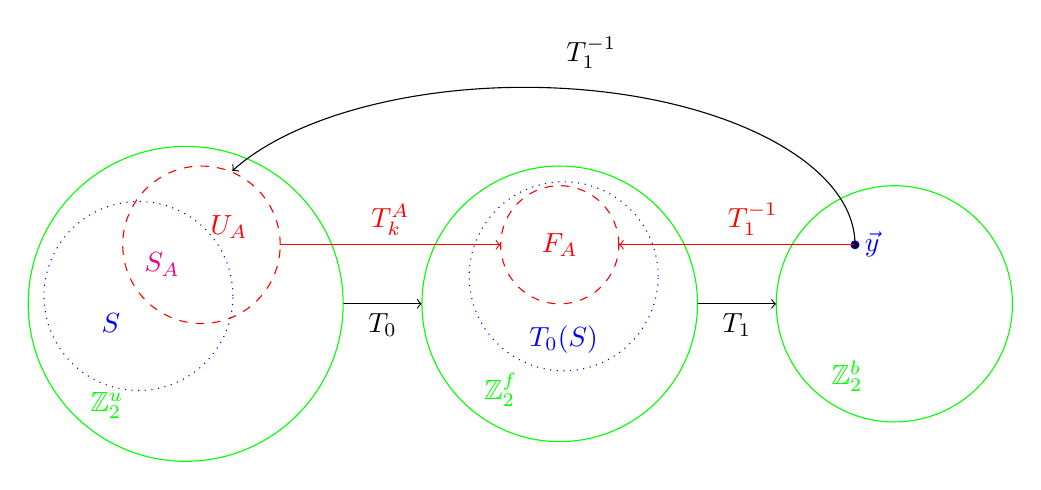
\begin{tikzpicture}
		\draw[->] (4,2) -- (5,2) node[left=0.5cm,below] {$T_0$};
		\draw[green] (2,2) circle (2cm) node[left=1cm,below=1cm] {$\binvecspace{u}$};
		\draw[green] (6.75,2) circle (1.75cm) node[left=0.75cm,below=0.75cm] {$\binvecspace{f}$};
		\draw[->] (8.5,2) -- (9.5,2) node[left=0.5cm,below] {$T_1$};
		\draw[green] (11,2) circle (1.5cm) node[left=0.6cm,below=0.6cm] {$\binvecspace{b}$};
		
		\draw[blue] (10.5,2.75) circle (0.05cm) [fill=black] node[anchor=west] {$\vec{y}$};
		\draw[->,red] (10.5,2.75) -- (7.5,2.75) node[left=-1.7cm,above] {$T_1^{-1}$};
		\draw[dashed,red] (6.75,2.75) circle (0.75cm) node[] {$F_A$};
		\draw[dotted,blue] (6.8,2.35) circle (1.2cm)  node[left=0cm,below=0.5cm] {$T_0(S)$};

		\draw[dashed,red] (2.2,2.75) circle (1cm)  node[left=-0.35cm,below=-0.5cm] {$U_A$};
		\draw[dotted,blue] (1.4,2.1) circle (1.2cm)  node[left=0.35cm,below=0.1cm] {$S$};

		\draw[->] (10.5,2.75) arc (0:152:4.2cm and 2cm) node[below=-1.5cm,left=-5cm] {$T_1^{-1}$};
		
		\draw[magenta] (1.7,2.5) node[] {$S_A$};
				
		\draw[->,red] (3.2,2.75) -- (6,2.75) node[left=1.4cm,above] {$T_k^A$};
	\end{tikzpicture}
\end{center}
\end{figure}

\begin{corollary}
\label{corollary-e1-e2}
For each $\epsilon > 0$ there is $c_\epsilon > 0$ such that if $l \geq c_\epsilon (f - b)2^{f-b}$, then
\[
\probs{T \in_U \linearmaps{u}{b}}{E_1} \leq \frac{1}{1 - \epsilon}\probs{T_0 \in_U \linearmaps{u}{f}, T_1 \in_U \surjectivelinearmaps{f}{b}\colon T = T_0 \circ T_1}{E_2}
\]
\end{corollary}
\begin{proof}
$1- \epsilon \leq \prob{E_2 | E_1} \leq \frac{\prob{E_2}}{\prob{E_1}}$.
This bound holds for each choice of $T_0$, $T_1$ with the uniform choice of $T_k$. Hence it must hold for the complete uniform choice of $T_0$, $T_1$ because it gives the uniform choice of $T_k$.
\end{proof}

\begin{lemma}
\label{lemma-bound}
If $S \subseteq \binvecspace{u}$, $|S| = 2^b$ and $\mu = \frac{|S|}{|\binvecspace{f}|} = 2^{b - f}$, then
\[
\probs{T_0 \in_U \linearmaps{u}{f}, T_1 \in_U \surjectivelinearmaps{f}{b}}{E_2(S, T_0, T_1)} \leq \mu ^ {-\log b - \log \mu + \log \log \mu^{-1}}.
\]
\end{lemma}
\begin{proof}
It is possible to restate the occurrence of $E_2(S, T_0, T_1)$ as $T_1(\binvecspace{f} - T_0(S)) \neq \binvecspace{b}$ since $E_2(S, T_0, T_1)$ occurs iff $\exists \vec{y} \colon \vec{y} \not\in T_1(\binvecspace{f} - T_0(S))$.
We use Theorem~\ref{theorem-prob-bound} for $T_1$, $\binvecspace{f} - T_0(S)$, source space $\binvecspace{f}$ and target space $\binvecspace{b}$.
In our case we have $\alpha = 1 - \frac{|\binvecspace{f} - T_0(S)|}{|\binvecspace{f}|} \leq \frac{|T_0(S)|}{2^f} \leq \frac{|S|}{2^f} \leq \mu$.
Hence
$
\prob{E_2(S, T_0, T_1)} \leq \alpha ^ {f - b - \log b + \log \log \alpha^{-1}} \leq \mu ^ {-\log \mu - \log b + \log \log \mu^{-1}}.
$
For the last inequality observe that the function $\alpha ^ {f - b - \log b + \log \log \alpha^{-1}}$ is increasing w.r.t. $\alpha$ in $(0, 1)$.
\end{proof} 

\begin{theorem}
\label{theorem-prob-distribution-bound}
Let $r > 4$. Then
\[
\probs{T \in_U \linearmaps{u}{b}}{\lbin{T}{S} \geq 2 c_\epsilon r} \leq \frac{1}{1 - \epsilon}\left(\frac{\log r}{r}\right)^{-\log b - \log \frac{\log r}{r} + \log \log \frac{r}{\log r}}.
\]
\end{theorem}
\begin{proof}
From definition of $E_1$ we have that $\lbin{T}{S} \geq 2 c_\epsilon r$ occurs whenever $E_1(S, T, 2 c_\epsilon r)$ occurs.
To bound the probability of $E_1(S, T, 2 c_\epsilon r)$ we bound $\prob{E_2(S, T_0, T_1)}$ for a suitable chosen factor space $\binvecspace{f}$.
We put $f = \lfloor b + \log r - \log \log r + 1 \rfloor$ and $l = 2c_\epsilon r$.

The choice of $f$ meets the requirement $f \geq b$ of Corollary~\ref{corollary-e1-e2} and Lemma~\ref{lemma-bound}, i.e. $\surjectivelinearmaps{f}{b}$ is nonempty.

In Corollary~\ref{corollary-e1-e2} we also assume that $l \geq c_\epsilon (f - b)2^{f - b}$.
For $r \geq 4$ we have $(f - b)2^{f - b} \leq (\log r - \log \log r + 1)2^{\log r - \log \log r + 1} \leq \frac{2r(\log r - \log \log r + 1)}{\log r} \leq 2r$ and thus this assumption is met.

Use Lemma~\ref{lemma-bound} with $\mu = 2^{b - f} \leq \frac{\log r}{r}$ and the fact that $f(\mu) := \mu ^ {- \log b + \log \mu^{-1} + \log \log \mu^{-1}}$ is increasing in $(0, 1)$.
Hence $\prob{E_2(S, T_0, T_1)} \leq f(\mu) \leq f(\log r/r)$.
Bounding $\prob{E_1}$ using Corollary~\ref{corollary-e1-e2} yields the statement.
\end{proof}

We prove Theorem~\ref{theorem-n-to-n}.
\begin{proof}[Proof of Theorem~\ref{theorem-n-to-n}]
The idea is simple, we bound $\sum_{l = 4\log n}^{b} \probs{T\in_U\linearmaps{u}{b}}{\lbin{T}{S} \geq l}$ by a constant.
We show that if $r \geq 4b = 4\log n$, then the probability of having a chain longer then $2 c_\epsilon r$ is bounded from above by $r^{-1.5}$.
The exponent in the bound from Theorem~\ref{theorem-prob-distribution-bound} may be bounded as
\[
-\log b - \log \log r + \log r + \log (\log r - \log \log r) \geq -\log \log r + 2 + \log \left(\frac{3\log r}{4}\right) \geq \log(3).
\]
Finally for $r \geq 4\log n$ we may conclude that $\prob{\lbin{T}{S} \geq 2c_\epsilon r} \leq \left(\frac{\log r}{r}\right)^{\log 3} \leq r^{-1.5}$ and hence $\int_{r = 4\log n}^{n} \prob{\lbin{T}{S} \geq 2c_\epsilon r} \operatorname{d}r = O(1)$ and hence the above sum is convergent.
\end{proof}

\section{A special case when $S$ is a vector subspace}

Now we bound the size of the largest bin when $S$ is a subspace of the universe.
We first notice that the bins have a simple structure -- all of them are formed by elements which are affine subspaces of the universe.
This means that bins have the same size and in addition the bin of vector $0$ in $\binvecspace{2}$ always exists and is a largest bin of expected constant size.

\begin{theorem}
Let $b, u \in \mathbb{N}$ and $v_1, \dots, v_b \in \mathbb{Z}_2^u$ be linearly independent. Then \[ \expects{h \in_U \linearmaps{u}{b}}{\lbin{h}{\operatorname{Span}(v_1, \dots, v_b)}} = O(1) .\]
\end{theorem}
\begin{proof}
For convenience put $S = \operatorname{Span}(v_1, \dots, v_b)$. 
We show that each non-empty bin created by a transformation $h$ is formed by balls from an affine subspace of $S$ and has the size of the kernel of $h$.
From this it follows that $\expect{\lbin{h}{S}} = \expect{\bin{h}{S}{0}} = O(1)$.

Without loss of generality assume that $v_1, \dots, v_k$ are the vectors forming the kernel of $h$, i.e. $h(v_i) = 0$ where $i \in \{1, \dots, k\}$.
If $h(v) = y$ for some $v \in S$, then $h^{-1}(y) \cap S = v + \operatorname{Span}(v_1, \dots, v_k)$.
Hence for each $y \in \mathbb{Z}_2^b$ it holds hat $|h^{-1}(y) \cap S| = 0 \vee |h^{-1}(y) \cap S| = 2^k$.
Thus the sizes of all the non-empty bins are the same and are equal to $\bin{h}{S}{0}$.
\end{proof}

We present a different proof of this property coming from the following ideas.
Notice that the structure of the bins can give an upper bound of having $l$ colliding elements.
The fact that we can find a bin which is always present avoids using the union bound.

\begin{theorem}
\label{theorem-bound-general}
If $A \subseteq \binvecspace{b}$, $\alpha_0 = 1 - |A|/2^b$, then \[\probs{f_1, \dots, f_b \in_U \binvecspace{b}}{1 - |A \cup (A + \operatorname{Span}(f_1, \dots, f_b)|/2^b \geq \mu} \leq \alpha_0^{b - \log \log \mu^{-1} + \log \log \alpha_0^{-1}}.\]
\end{theorem}
\begin{proof}
In~\cite{alonetal}.
\end{proof}

There is a chain of length at least $2^l$ iff $\operatorname{dim}(\operatorname{Ker}(T)) \geq l$, i.e. $\operatorname{rank}(T) < b - l$.
Let $e_1, \dots, e_b$ be the canonical basis of $\binvecspace{b}$. For each $e_i$ mapping  $T$ choses its image $f_i \in_U \binvecspace{b}$.
Mapping $T$ has rank less than $b - l$ iff $|\operatorname{Span}(f_1, \dots, f_b)| < 2^{b - l}$, i.e. $1 - |\operatorname{Span}(f_1, \dots, f_b)|/2^b > 1 - 2^{-l}$.
In our setting it holds $T(S) = \operatorname{Span}(f_1, \dots, f_b)$.
Hence $\lbin{T}{S} \geq 2^l$ iff $1 - |\operatorname{Span}(f_1, \dots, f_b)|/2^b > 1 - 2^{-l}$.

If we directly apply Theorem~\ref{theorem-bound-general} for $A = \{\vec{0}\}$ and the vectors $f_1, \dots, f_b$ chosen by $T$ we get the following estimate:
\[
\probs{}{\lbin{T}{S} \geq 2^l} \leq (1 - 2^{-b})^{b - \log (-\log (1 - 2^{-l})) + \log (-\log (1 - 2^{-b}))} \approx (1 - 2^{-b})^{b + l - b} \leq (1-2^{-b})^{l}.
\]
This is not sufficient to get $O(1)$ bound since the bound provided by Theorem~\ref{theorem-bound-general} for $\alpha_0$ close to $1$ is not tight.
Consider $A = \{\vec{0}\}$, i.e. $\alpha_0 = 1 - 2^{-b}$ and we add a single random vector $\vec{v}$ to $A$, i.e. $\alpha_1 = 1 - |A \cup (A + \vec{v})|/2^b$, then $\probs{v\in_U\binvecspace{b}}{\alpha_1 \geq 1 - 2^{-b}} = 2^{-b}$ since this is equivalent to $v = \vec{0}$.
From Theorem~\ref{theorem-bound-general} we get only
\[
\probs{v\in_U\binvecspace{b}}{\alpha_1 \geq 1 - 2^{-b}} \leq \alpha_0^{1 - \log \log \alpha_0^{-1} + \log \log \alpha_0^{-1}} = 1 - 2^{-b}.
\]
Compare $2^{-b}$ to the bound $1-2^{-b}$ obtained from the direct application of Theorem~\ref{theorem-bound-general}.

To get a sufficient result we use factorization similar to the one used in the proof of Theorem~7a in~\cite{alonetal}. It ensures that $\alpha_0$ is large enough.
First we bound the probability of having many collisions under a universal function $T$ following from using CSB and Markov inequalities.
This is a generalization of the well-known property of universal functions saying that $\probs{T \in_U \linearmaps{u}{b}}{\mbox{number of collisions created by }T \geq \frac{k}{2^b} \binom{|S|}{2}} \leq \frac{1}{k}$.
\begin{lemma}
\label{lemma-collisions-general}
\[
\probs{T \in_U \linearmaps{u}{b}}{|T(S)| \leq \frac{|S|}{k}} \leq \frac{|S| - 1}{(k - 1)2^b} \leq \frac{|S|}{k2^b}.
\]
\end{lemma}
\begin{proof}
Use CSB to bound the number of collisions from below and then use Markov inequality to obtain the probability bound.
\end{proof}

Now we switch back to bounding the probability of having a long chain.
We factor through a vector space $F$ of dimension $b$, i.e. the dimension of both source and target space.
The factorization is as usual, $T = T_0 \circ T_1$ where $T_1$ is surjective.

\begin{align*}
& \probs{T \in_U \linearmaps{u}{b}}{|T(S)| \leq 2^{b - l}} \\
& \quad \leq \probs{T \in_U \linearmaps{u}{b}}{|T(S)| \leq 2^{b - l} \wedge |T_0(S)| \leq 2^{b - \sqrt{l}}} + \probs{T \in_U \linearmaps{u}{b}}{|T(S)| \leq 2^{b - l} \wedge |T_0(S)| > 2^{b - \sqrt{l}}} \\
& \quad \leq \probs{T \in_U \linearmaps{u}{b}}{|T_0(S)| \leq 2^{b - \sqrt{l}}} + \probs{T \in_U \linearmaps{u}{b}}{|T(S)| \leq 2^{b - l} \mid |T_0(S)| > 2^{b - \sqrt{l}}}.
\end{align*}
Now by Lemma~\ref{lemma-collisions-general} we get
$
\probs{T \in_U \linearmaps{u}{b}}{|T_0(S)| \leq 2^{b - \sqrt{l}}} \leq 2^{-\sqrt{l}}.
$
Let us fix $T_0$ and denote $S_1 = T_0(S)$. From Theorem~\ref{theorem-bound-general} it follows that 
\[
\probs{T \in_U \linearmaps{u}{b}}{|T(S)| \leq 2^{b - l} \mid |T_0(S)| > 2^{b - \sqrt{l}}} = 
\probs{T_1 \in_U \surjectivelinearmaps{f}{b}}{|T_1(S_1)| \leq 2^{b - l} \mid |S_1| > 2^{b - \sqrt{l}}}.
\]
Directly use the following fact used in the proof of Theorem~7b in \cite{alonetal}.
Let $A \subseteq \binvecspace{u}$, $\alpha = 1 - |A|/2^u$
\[
\probs{T \in_U \surjectivelinearmaps{u}{b}}{1 - |T(A)|/2^b \geq 1 - 2^{-l}} \leq \alpha^{u - b - \log \log \left(1 - 2^{-l}\right)^{-1} + \log \log \alpha^{-1}}.
\]
Since $-2^{-l} \geq \log(1 - 2^{-l})$ we get
$
\probs{T \in_U \surjectivelinearmaps{u}{b}}{1 - |T(S)|/2^b \geq 1 - 2^{-l}} \leq \alpha^{u - b + l + \log \log \alpha^{-1}}.
$
In our case we have $u := b$, $b := b$, $T := T_1$, $A := S_1$ and $\alpha \leq 1-2^{-\sqrt{l}}$.
Moreover whenever $l \geq 2$, we have that $-2^{-l/2 + 1} \leq \log (1 - 2^{-l/2})$ and $1-2^{-\sqrt{l}} \leq e^{-\log(2)\sqrt{l}} \leq 2^{-\sqrt{l}}$.
Finally
\begin{align*}
& \probs{T_1 \in_U \surjectivelinearmaps{f}{b}}{|T_1(S_1)| \leq 2^{b - l} \mid |S_1| > 2^{b - 2\log l}} \\
& \quad = \probs{T_1 \in_U \surjectivelinearmaps{f}{b}}{1 - |T_1(S_1)|/2^b \geq 1 - 2^{-l} \mid |S_1| > 2^{b - 2\log l}} \\
& \quad \leq \left(1 - 2^{-2\log l}\right)^{l + 1 - l/2} \leq e^{-2^{-\sqrt{l}}(l/2 + 1)} \leq e^{-\sqrt{l}/2}.
\end{align*}

\section{Natural set for the multiply-shift system}

\begin{definition}[Mutliply-shift system]
Let $k, b \in \mathbb{N}$, $k \geq b$ and $a \in [2^k]$, $2 \nmid a$.
Let the function $h_a \colon [2^k] \to [2^b]$ map $x$ to $h_a(x) =(ax \bmod 2^k) \div 2^{k - b}$.
The system $\mathcal{MS}_{k}^{b} = \{h_a \mid a \in [2^k], 2 \nmid a\}$ is called \emph{multiply-shift system}.

\end{definition}

Let $m = 2^b$.
The best possible case is when $S = [m] + 2^{k} - m$. Then there is no function which creates a collision on such a set.
The elements of $S$ are number with the $k-b$ significant bits equal to zero.

Let $x, y \in S$, $x \neq y$. Observe that for any $a \in [2^k]$, $2 \nmid a$, we have $ax \bmod 2^k \neq ay \bmod 2^k$ and the $k - b$ least significant bits of both values are zeros.
Hence $h_a(x) \neq h_a(y)$.

We can prove $\expect{\vlbin{S}} = O(1)$ for $S = [m]$.
Let us note that for an odd $a$ the sets $[m]$ and $a[m]$ have the same behavior with respect to $\mathcal{MS}_{k}^{b}$ since multiplication by an odd number just permutes the functions.
From this it follows that for any $a \in [2^k]$, $2 \nmid a$ and $S = a[m]$ we get the same expectation as for $S = [m]$. 
\begin{lemma}
When $k \geq 2b$ and $S = [2^b]$, then $\expect{\vlbin{S}} = O(1)$.
\end{lemma}
\begin{proof}
Let $y \in [2^b]$, then $h_a^{-1}(y) = (a^{-1} (y + [2^{k - b}])) \bmod 2^k$ where the inverse of $a$ is taken in $[2^k]$.
\begin{claim}
Let $\operatorname{GCD}(g, 2^k) = 1$, then $g(y + [2^{k - b}]) \bmod 2^{k} \cap [2^b]$ is a union of at most two arithmetic progressions.
\end{claim}
\begin{proof}
If $g < 2^b$, then the claim holds since $g2^{k - b} < 2^k$. The shift by $yg$ can split the arithmetic progression with the difference $g$ intersecting with $[2^{b}]$ into at most two progressions.

If $g > 2^b$, then from the assumption that $k \geq 2b$  we get that the elements in the intersection are the first elements from the leaps over $2^k$. We use an inductive argument on the first elements of leaps intersecting the input set, i.e. $((-2^k) \bmod a) [ma/2^k] \cap [2^b]$.
\end{proof}

\begin{itemize}
 \item The longest chain is always formed with $0$ as its smallest element.
 \item Probability of collision of an arithmetic progression of length $l$ into a single element
\end{itemize}
\end{proof}

\section{Natural set for linear functions modulo prime}

\begin{thebibliography}{32}
\bibitem{alonetal}
N. Alon, M. Dietzfelbinger, P. B. Miltersen, E. Petrank and G. Tardos
\newblock Linear Hash Functions
\newblock J. {ACM}, 46. pages 667--683, 1999

% \bibitem{cw}
% J.L. Carter, and M.N. Wegman. 
% \newblock Universal Classes of Hash Functions.
% \newblock Journal of Computer and System Sciences, 18. pages 143--154, 1979.

% \bibitem{siegel}
% A. Siegel. 
% \newblock On universal classes of extremely random constant-time hash functions
% \newblock SIAM Journal on Computing, 33(3). pages 505--543 (electronic), 2004

% \bibitem{wieder}
% L.E. Celis, O. Reingold, G. Segen, and U. Wieder
% \newblock Balls and Bins: Smaller Hash Families and Faster Evaluation
% \newblock Foundations of Computer Science (FOCS), 2011 IEEE 52nd Annual Symposium, pages 599 -- 608, 2011

% \bibitem{azar}
% Y. Azar, A. Broder, A. Karlin, and E. Upfal
% \newblock Balanced allocations.
% \newblock SIAM Journal on Computing, 29(1). pages 180--200, 1999.

% \bibitem{vocking}
% B. V\"{o}cking
% \newblock How asymmetry helps load balancing.
% \newblock In Proceedings of the Fortieth Annual Symposium on Foundations of Computer Science. pages 131--140, 1999.
\end{thebibliography}

\end{document}


 
